\chapter{Wykonanie projektu}
\label{cha:course}

\section{Projekt płytki}
\subsection{Schemat}
Projekt płytki, naturalnie rozpoczęto od wykonania schematu ideowego. W tym celu przyjęto następujące założenia:
\begin{itemize}
    \item Układ, musi być zasilany zewnętrznie (5v oraz 3.3V)
    \item Wykorzystany zostanie konwerter UART-USB
    \item Układ, będzie można wyłączyć tranzystorem, sterującym przetwornicami
    \item Wykorzystany zostanie zewnętrzny generator
\end{itemize}
Według standardu mikroBUS\texttrademark, płytka zasilana jest przez układ w który jest wpięta. Często jest to zasilanie procesora, na którym tworzone jest oprogramowanie. Ponieważ w opisywanym projekcie, wykorzystany został procesor, oraz trzy sensory (w tym jeden pracujący z napięciem 5V), zdecydowano się na zasilanie zewnętrzne. Miało ono zminimalizować prawdopodobieństwo nieprawidłowej pracy układu. Jednocześnie, czujnik MQ2 pobierając setki mA prądu, mógłby uszkodzić przetwornicę układu w który została wpięta płytka. Najprostszym rozwiązaniem, było wyprowadzenie portu USB i zasilanie z niego układu. Zwrócono uwagę na fakt, że USB w komputerach, nie ma stabilnego napięcia 5V, a często wręcz 4.7-4.8V. Jest to zachowanie zdefiniowane w standardzie USB 2.0 \cite{usb_specification} w rozdziale 7. Z tego powodu , należało wykorzystać regulator napięcia. \newline Wybór tego i wszystkich kolejnych komponentów, podyktowany był w dużej mierze dostępnością na rynku. Kolejnym kryterium, były parametry układu, opisywane w dostarczanych przez producentów dokumentacjach. Jako układ do zasilania sensora MQ2, wykorzystano przetwornicę typu BOOST - MCP1642 o wyjściowym napięciu właśnie 5V. Pozwoliła ona na stabilne zasilenie czujnika. Jej ważną cechą, jest maksymalny prąd na wyjściu, o wartości 800mA\cite{mq2_datasheet}. Wysoki prąd jest tutaj niezbędny, ponieważ zasilanie wspomnianego czujnika wymaga nawet 200mA prądu stałego. Do zasilania reszty elementów, wykorzystano regulator LDO  MIC5365 o wyjściowym napięciu 3.3V\cite{mic_datasheet}. Gwarantowany prąd wyjściowy regulatora to 150mA, co jest wartością wystarczającą do zasilenia reszty elementów z zapasem. Całość, z założenia włączana miała być tranzystorem NMOS 2N7002. Bramka tego tranzystora, połączona jest z pinem RESET standardu mikroBUS\texttrademark, pozwalając użytkownikowi wyłączyć układ. W przypadku tego elementu, pojawiły się dwa błędy, wymagające przerobienia gotowej płytki. Problem, szerzej opisano w podrozdziale \ref{sub:mistakes}. \newline
Schemat oraz layout, wykonane zostały w programie KiCad. Opensourcowym oprogramowaniu dla różnych systemów operacyjnych. Program ten, umożliwia podział schematu na bloki, co wykorzystano przenosząc sekcję zasilania do osobnego schematu. Na schemacie \ref{img:power_sch} przedstawiono całą, wspomnianą sekcję. Zasilanie, doprowadzone jest z USB do obu przetwornic. Gdy procesor jest zasilony, a więc działa przetwornica 3.3V, włączona zostaje czerwona dioda LED. Widoczny na schemacie rezystor R10, nie jest uwzględniony w layoucie i został dołożony ręcznie do płytki. Więcej na ten temat, opowiada podrozdział \ref{sub:mistakes}.
\newline Na schemacie, widoczna jest również znacząca ilość kondensatorów. Zostały one dodane do schematu, jako wskazane przez producenta jako konieczne dla poprawnego działania układów. Bardzo istotny jest również rezystor R7, gwarantujący ustalony stan niski po wyłączeniu tranzystora.
\begin{figure}[H]
    \centering
    \includegraphics[width=\textwidth, height=\textheight, keepaspectratio]{Graphics/power_sch.png}
    \caption{Schemat części zasilającej moduł}
    \label{img:power_sch}
\end{figure}
Kolejnym blokiem, jest schemat \ref{img:sensors_sch}, zawierający w sobie wszystkie czujniki. Podobnie jak wcześniej, producenci w swoich dokumentacjach zalecają stosowanie kondensatorów, jak najbliżej zasilania układu, dla zapewnienia jego prawidłowego działania. W przypadku sensora działającego z użyciem SPI - BMP280 - zastosowano rezystor pull-down na linii MISO\cite{bmp_datasheet}. Dzięki temu, gdy linia nie jest używana, zagwarantowany jest stan niski. Podobnie w przypadku linii NSS. Zastosowanie rezystora podciągającego do zasilania, pozwala zagwarantować, że układ nie będzie aktywny gdy nie jest to pożądane.\newline
Wartym uwagi jest układ czujnika analogowego MQ2. Ze względu na zastosowany procesor, mierzone przetwornikiem napięcie, musi mieścić się w przedziale 0-3.6V. Ponieważ wybrany czujnik działa w zakresie 0-5V, konieczne jest zastosowanie dzielnika napięcia. W tym przypadku, układ rezytorów oraz czujnika, staje się źródłem prądu, który mógłby uszkodzić procesor. Z tego powodu, zastosowano wzmacniacz operacyjny w konfiguracji nieodwracającego wtórnika napięciowego. Wzmacniacz operacyjny, mający bardzo małą rezystancję wyjściową, stanowi w przybliżeniu źródło napięcia równe co do wartości spadkowi napięcia na R11.
\newline
\newline
Ostatnim, a zarazem najistotniejszym, jest schemat \ref{img:main_sch}. Po jego lewej stronie, zaznaczono fragment odpowiadający za konwersję UART-USB. Wykorzystany układ konwertera to CP2102\cite{cp2102_datasheet}. Układ ten, pozwala obserwować logi mikroprocesora przy użyciu tego samego przewodu, którym zasilamy płytkę. W trakcie tworzenia schematu, rozważano również tylko wyprowadzenie testpointów, pozwalających na podejrzenie logów zewnętrznym konwerterem. Ponieważ jednak planowany jest również inny projekt, wykorzystujący wiele takich konwerterów, zdecydowano się na jego użycie w celach przede wszystkim edukacyjnych i testowych. Głównym zagadnieniem z nim z związanym, było użycie pary różnicowej, wymaganej dla prawidłowegodziałania USB.
\newline
Po prawej stronie schematu \ref{img:main_sch}, widoczny jest blok mikroprocesora STM32F103C8. Zastosowano tutaj zewnętrzny generator o taktowaniu 8MHz, zastępując wewnętrzny zegar mikroprocesora. Istotnym zaganieniem, wymaganym przez mikroprocesor według dokumentacji, jest montaż osobnych kondensatorów o wartości 100n przy każdym z pinów zasilania, możliwie jak najbliżej układu. Dla zapewnienia prawidłowego działania magistrali I$^2$C, dodano rezystory podciągające linie do zasilania. Wszystkie piny posiadają też testpointy, mające ułatwić tworzenie oprogramowania dzięki szybkiemu wykryciu błędów w transmisji, a więc np. w zlutowaniu układu. Dodatkowo, na pinie 8, wyprowadzono LED. Zgodnie z przyjętymi przez zespół założeniami, wskazuje on gotowość układu do pracy, a więc przejście wszystkich kroków inicjalizacyjnych.
\newline
Wartym zaznaczenia jest tutaj fakt nie wyprowadzenia pinów SWDIO oraz SWCLK. Ponieważ są to piny wymagane tylko na etapie tworzenia oprogramowania, podjęto decyzję o ich niewykorzystaniu. Ważną w tym wypadku kwestią, był również brak miejsca na ścieżki, pozwalające na taki zabieg. Niemniej jednak, osoba składająca PCB, bez większych problemów była w stanie wlutować przewody programatora bezpośrednio do pinów mikroprocesora.
\begin{figure}[H]
    \centering
    \includegraphics[width=\textwidth, height=\textheight, keepaspectratio]{Graphics/sensors_sch.png}
    \caption{Schemat połączeń czujników}
    \label{img:sensors_sch}
\end{figure}
\begin{figure}[H]
    \centering
    \includegraphics[width=\textwidth, height=\textheight, keepaspectratio]{Graphics/main_sch.png}
    \caption{Schemat połączeń konwertera UART-USB oraz mikroprocesora}
    \label{img:main_sch}
\end{figure}

\subsection{Layout}
W kolejnym kroku, wykonany został layout płytki. Obrazek \ref{img:front_layout} przedstawia frontową warstwę elektryczną płytki oraz nadruki na niej. Z założenia, jest to warstwa w większości wypełniona masą (GND). Niestety, ze względu na brak miejsca na warstwie tylnej, masa układu jest znacząco pocięta, choć pozostaje jednolita. W przypadku linii 5V, zasilającej czujnik MQ2, zasosowano znacznie szersze ścieżki o szerokości 30mils. Pozostałe, mają szerokość 12 oraz 7,87mils. Druga z tych wartości, jest wartością minimalną, domyślną dla programu KiCad. Mimo ręcznego ustawiania mniejszej szerokości, zgodnej z zaleceniami JLCPCB\cite{jlcpcb_specification}, program automatycznie zmieniał szerokość ścieżki na większą. Podobnie było w przypadku przelotek. Niestety, zorientowano się o tym pod koniec tworzenia płytki, a mogłoby to pomóc oszczędzić miejsce. Szczególnie istotne, jest to dla warstwy sygnałowej, przedstawionej na rysunku \ref{img:back_layout}. Ze względu na czytelność, rysunek przedstawia jedynie połączenia elektryczne, bez nadruku. Jako elementy pasywne, wykorzystano te w obudowach 0806 oraz pojedyncze elementy 0402. Również w przypadku tej warstwy, znacząco pogrubiono ścieżki doprowadzające zasilanie. Ma to na celu poprawę przewodności ścieżek, która zeleży od ich szerokości. Jak można zauważyć, na płytce jest bardzo gęsto, a część elementów znajduje się na granicy spełnienia warunków DRC (np. odstępów między padami). Ponieważ jednak był to pierwszy projekt płytki autora, popełniono tutaj kilka błędów. Najważniejszym z nich, jest użycie komponentów 0806. Zdecydowano się na nie, ponieważ wszystko lutowane było ręcznie (z użyciem szablonu do pasty, jednak w trakcie wykonywania projektu, większość układów była wielokrotnie ręcznie przelutowywana). Niestety, zajmują one bardzo dużo miejsca na płytce, a obudowy 0603 również dają się łatwo lutować ręcznie. Dobrą zmianą, byłaby również bardziej zwarta sekcja zasilania. Dodatkowe miejsce, mogłoby pozwolić wygodniej umiejscowić komponenty. Również szerokość ścieżek sygnałowych, mniejsza o 1,87mils (0,0254mm) mogłaby pozwolić zaoszczędzić nieco miejsca i lepiej poprowadzić ścieżki.
\newline
Po wygenerowaniu plików, płytkę oraz szablon, zamówiono w serwisie JLCPCB. Jednocześnie, części zamówiono w sklepie Mouser. Obrazek \ref{img:pcb_photo} przedstawia gotową, wykonaną płytkę przed przylutowaniem elementów. Natomiast obrazek \ref{img:pcb_rdy_photo} przedstawia zlutowaną, gotową płytkę przed wykonaniem niezbędnych przeróbek, omówionych w następnym podrozdziale. 

\begin{figure}[H]
    \centering
    \includegraphics[width=\textwidth, height=\textheight, keepaspectratio]{Graphics/pcb_front.png}
    \caption{Frontowa warstwa elektryczna płytki}
    \label{img:front_layout}
\end{figure}

\begin{figure}[H]
    \centering
    \includegraphics[width=\textwidth, height=\textheight, keepaspectratio]{Graphics/pcb_back.png}
    \caption{Tylna warstwa sygnałowa płytki}
    \label{img:back_layout}
\end{figure}

\begin{figure}[H]
    \centering
    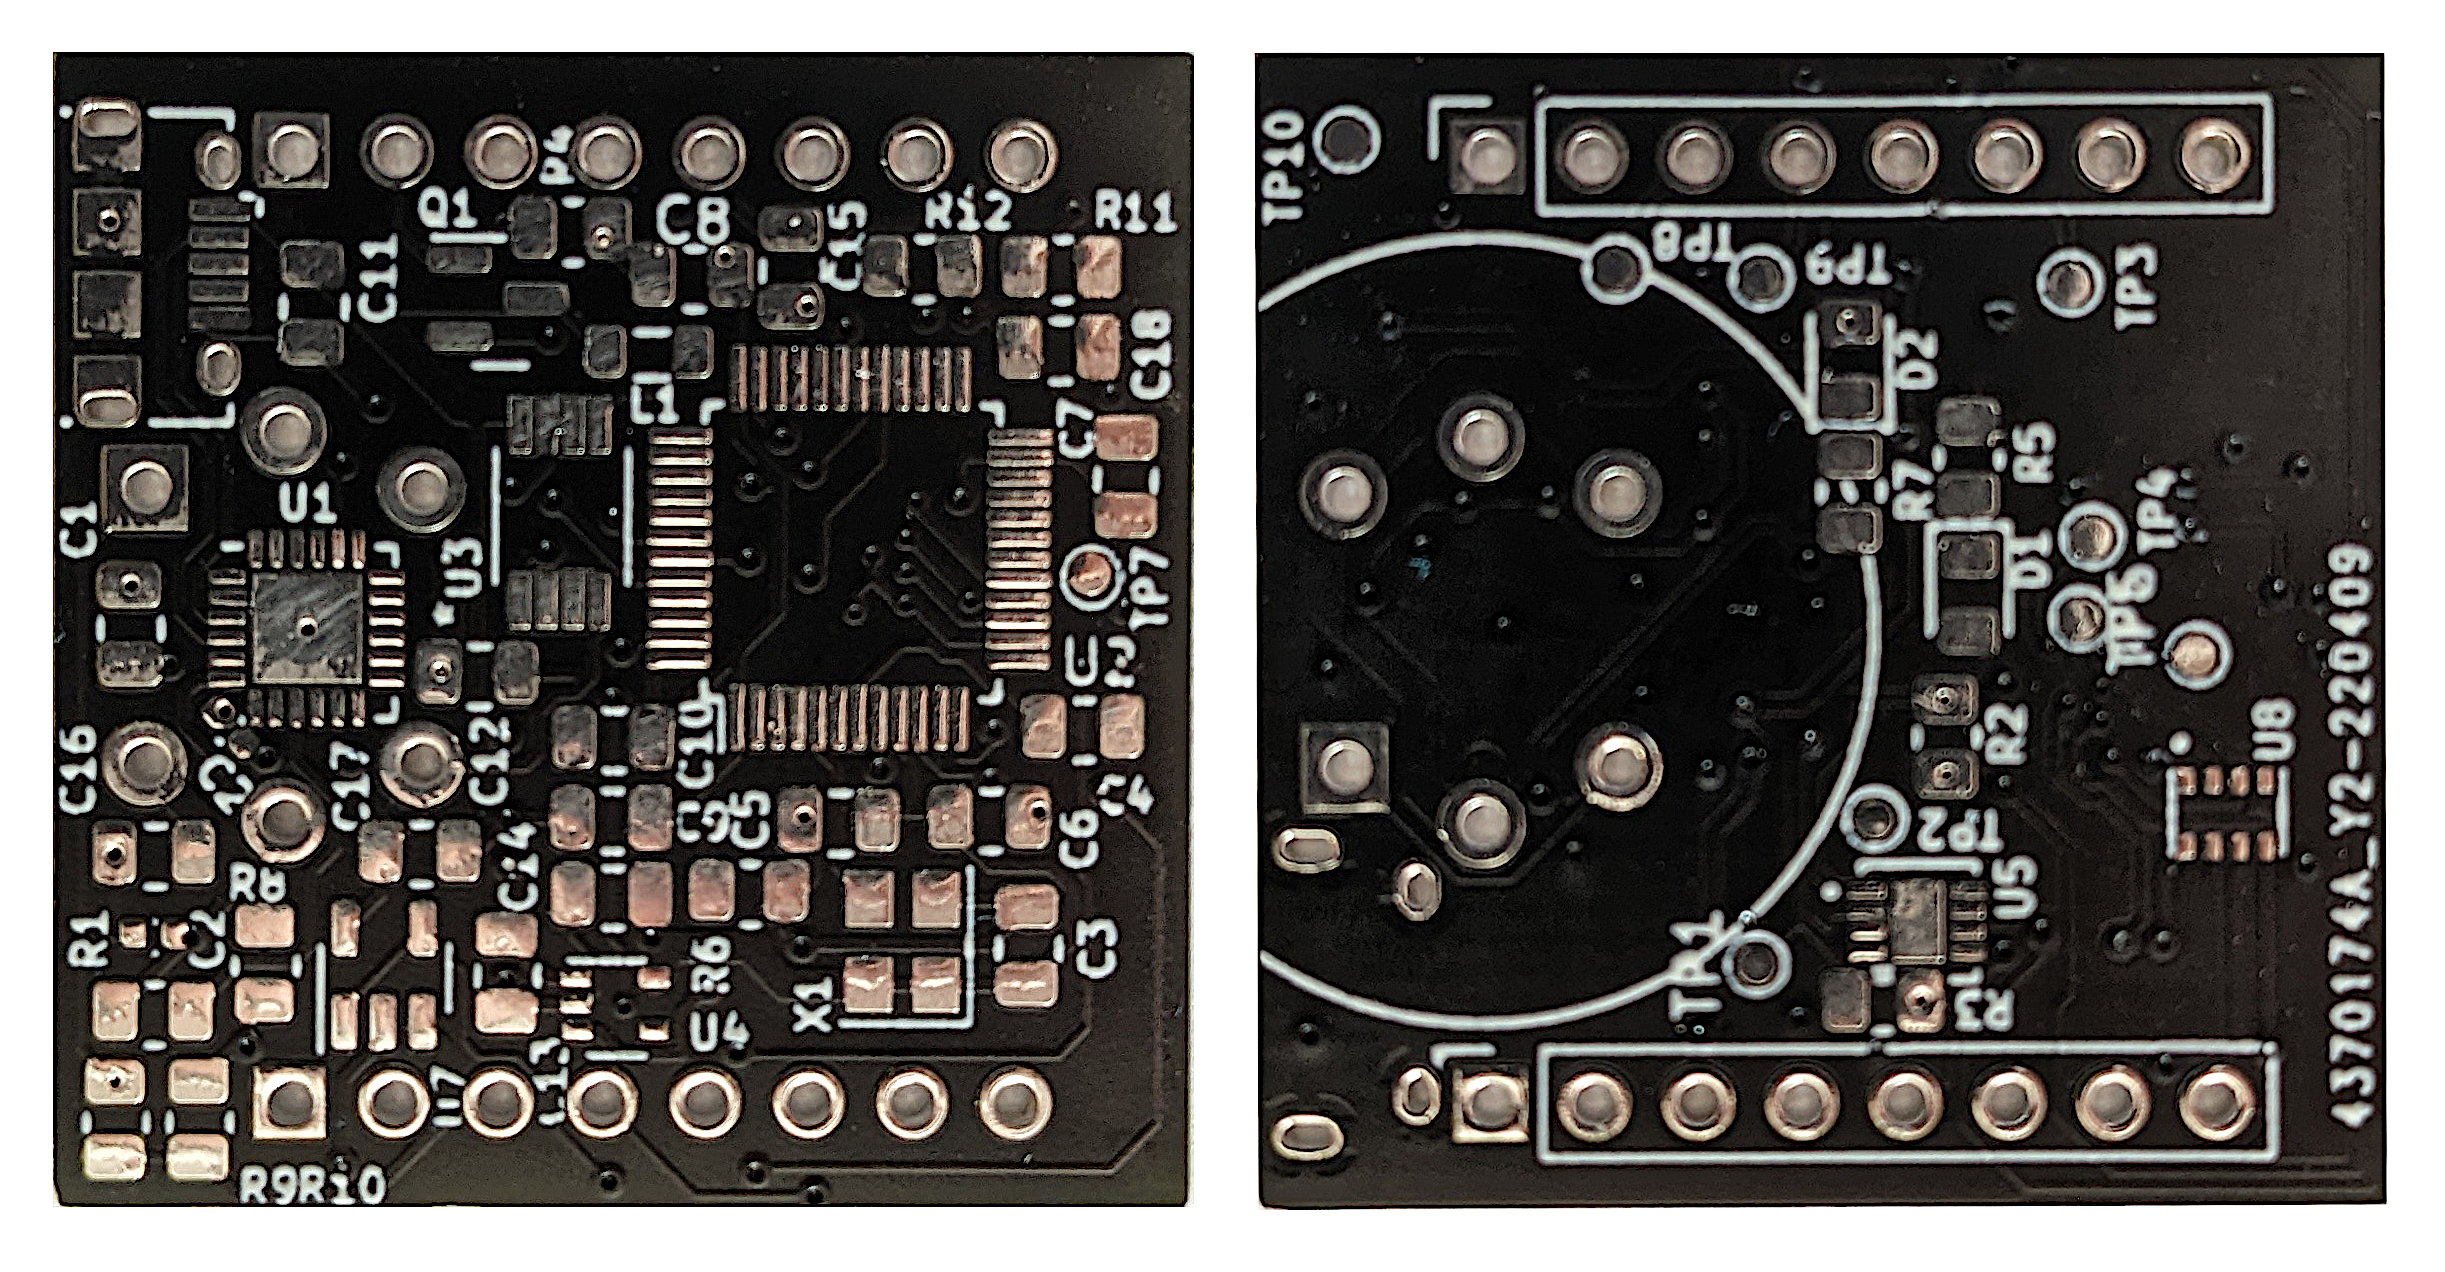
\includegraphics[width=\textwidth, height=\textheight, keepaspectratio]{Graphics/pcb_photo.png}
    \caption{Zdjęcie wykonanej płytki przed lutowaniem elementów}
    \label{img:pcb_photo}
\end{figure}

\begin{figure}[H]
    \centering
    \includegraphics[width=\textwidth, height=\textheight, keepaspectratio]{Graphics/pcb_rdy_photo.png}
    \caption{Zdjęcie wykonanej płytki po lutowaniu elementów}
    \label{img:pcb_rdy_photo}
\end{figure}

\subsection{Kompatybilność elektromagnetyczna}
W ramach ćwiczeń laboratoryjnych z przedmiotu Kompatybilność elektromagnetyczna wykonane zostały pomiary zaburzeń promieniowanych przez moduł. 
Rysunek \ref{img:emc_uc} przedstawia otrzymane wyniki w odniesieni do obowiązujących norm PN-EN55011 oraz PN-EN55022, które to określają
wymagania jakie muszą spełnić urządzenia, aby poprawnie działać w środowisku elektromagnetycznym. 

\begin{figure}[H]
    \centering
    \includegraphics[width=7cm]{Graphics/emc_hz530.jpg}
    \caption{Pomiar zaburzeń promieniowanych}
    \label{img:emc_hz530}
\end{figure}

W zależności od emitowanego poziomu zakłuceń, urządzenia można podzielić na 2 klasy (A i B). Klasa B jest przeznaczona głównie do zastosowań w środowisku mieszkalnym, czyli takim gdzie możemy spodziewać się odbiorników radiowych w odległości 10m. Klasa A zawiera w sobie urządzenia, które nie spełniają wymagań dla klasy B i tym samym mogą powodować zakłócenia radioelektryczne.

\begin{figure}[H]
    \centering
    \includegraphics[width=\textwidth, height=\textheight, keepaspectratio]{Graphics/emc_uc.jpg}
    \caption{Zakłucenia promieniowane - pomiar mikrokontrolera}
    \label{img:emc_uc}
\end{figure}

Bezpośrednia obserwacja zaburzeń emitowanych przez mikrokontroler pozwala zdiagnozować jeden z problemów urządzenia. Na rysunku \ref{img:emc_uc} widoczne są regularne piki oddalone od siebie o ok. 16MHz. Są to harmoniczne sygnału zegarowego 8MHz.
\newline
Sygnał prostokątny taktujący mikrokontroler możemy rozwinąć w następujący szereg Fouriera: 
\newline
$u(t) = \frac{4A}{\pi} (sin(wt)) + \frac{sin(3\omega t)}{3} + \frac{sin(5\omega t)}{5} + ... = \frac{4A}{\pi} \sum \limits_{i=1}^{\infty} \frac{sin((2k - 1)\omega t)}{2k - 1}$
\newline
Dlatego też widzimy jedynie nieparzyste wielokrotności częstotliwości bazowej. Dodatkowo zachowany jest stosunek mocy kolejnych pików. Zgodnie z teorią trzeci prążek powinien być o 9,54 dB (20log(1/3)) niższy od pierwszego, natomiast piąty o 13,97 dB (20log(1/5)).
\newline
Źródłem zaburzeń jest najprawdopodobniej zewnętrzny oscylator oznaczony na rysunku \ref{img:emc_clock} jako X1 (kolorem czerwonym oznaczono ścieżkę sygnału taktującego mikrokontroler).
\newline
Przekroczenie norm dla urządzeń klasy A nastąpiło dla trzeciej harmonicznej (40MHz), natomiast kolejne piki uniemożliwiają klasyfikację urządzenia jako typ B.

\begin{figure}[H]
    \centering
    \includegraphics[width=7cm]{Graphics/emc_clock.jpg}
    \caption{Zewnętrzny oscylator}
    \label{img:emc_clock}
\end{figure}

\subsection{Popełnione błędy oraz wykonane przeróbki}
\label{sub:mistakes}
Niestety, ze względu na zupełny brak doświadczenia w projektowaniu układów elektronicznych oraz zwykłe niedopatrzenia, popełniony został szereg błędów, wymagający zmian w celu uruchomienia płytki.
\newline \newline
Pierwszym z wykrytych błędów, była bramka tranzystora włączającego przetwornice wisząca w powietrzu. Zaznaczony na schemacie \ref{img:power_sch} rezystor R6, dodany został już po wyprodukowaniu płytek. Ze względu na jego brak, bramka znajdowała się w niaustalonym stanie, a mówiąc kolokwialnie - pływała. Powodowało to włączanie i wyłączenie układu w krótkich odstępach czasu, co uwidoczniło się przez mruganie diody LED po podpięciu zasilania, ale nie doprowadzeniu zasilania na bramkę tranzystora. Uruchomiony raz układ, nie wyłączał się, ponieważ zgromadzone w bramce ładunki, nie miały gdzie ujść. Rozwiązaniem było właśnie dodanie rezystora R6 ściągającego do masy. Rozwiązanie na fragmencie layoutu oraz złożonej płytce, przedstawia rysunek \ref{img:fix_gate}. Kolorem żółtym, zaznaczono istotne elementy, pozwalające odnaleźć miejsce na schemacie oraz layoucie, a kolorem zielonym, dodany element.

\begin{figure}[H]
    \centering
    \includegraphics[width=\textwidth, height=\textheight, keepaspectratio]{Graphics/fix_gate.png}
    \caption{Rezystor ściągający bramkę do masy}
    \label{img:fix_gate}
\end{figure}
Jak się później okazało, wspomniany mosfet generował znacznie więcej problemów. Najważniejszym z nich, było nie włączanie przetwornicy MCP1642. Aby przetwornica mogła być włączona, napięcie na pinie EN, powinno wynosić 0.75 * Vin\cite{mcp_datasheet}. W przypadku tego układu, wartość ta wynosi 3.5V. Niestety, w stworzonej konfiguracji, napięcie nie przekracza 1.5V. W trakcie realizacji projektu, podjęto kilka różnych prób przerobienia układu w taki sposób, aby przetwornica mogła zadziałać poprawnie. Wszystkie z nich, opisane zostały poniżej. Ostatecznie jednak, zdecydowano podłączyć pin EN na stałę do zasilania USB (Vbus). Nie niesie to za sobą znaczących konsekwencji, ponieważ przetwornica ta, zasila jedynie czujnik MQ2, a ten, jako czujnik analogowy, nie wymaga resetu. Obrazek \ref{img:fix_mcp1642} przedstawia zastosowaną poprawkę. Zielonym kolorem zaznaczono miejsce zwarcia ścieżki z pinem przetwornicy.
\begin{figure}[H]
    \centering
    \includegraphics[width=\textwidth, height=\textheight, keepaspectratio]{Graphics/fix_mcp1602.png}
    \caption{Zwarcie pinu EN ze ścieżką Vbus}
    \label{img:fix_mcp1642}
\end{figure}
Jedną z prób naprawienia układu, było przerobienie fragmentu z tranzystorem NMOS. Zmiany, przedstawiono na rysunku \ref{img:fix_gate_2}. Odcięto źródło tranzystora, a następnie zwarto je do masy. Tak samo jak w opisanym wcześniej przypadku, dodano rezystor ściągający bramkę do masy. Między dren a zasilanie, dodany został rezystor o wartości 1k$\Omega$. W tej konfiguracji, układ wyłączany byłby stanem wysokim, co rozwiązano w przykładzie poniżej. Niestety, przerobienie układu w ten sposób nie przyniosło zamierzonego efektu. Mała ilość miejsca wymusiła ręczne wlutowanie rezystora fizycznie pod tranzystor, a jednocześnie prawdopodobnie między wszystkimi cięciami i padami występowało jakieś niepożądane zwarcie. Niemniej jednak, w przypadku ponownej produkcji płytki, zmiana ta mogłaby być wprowadzona.
\begin{figure}[H]
    \centering
    \includegraphics[width=\textwidth, height=\textheight, keepaspectratio]{Graphics/fix_gate_2.png}
    \caption{Poprawiony schemat z użyciem tranzystora NMOS}
    \label{img:fix_gate_2}
\end{figure}
Powyższe rozwiązanie, ma zasadniczą wadę - układ domyślnie jest włączony. Sprawia to, że użytkownik zanim napisze fragment programu mogący sterować układem włączania i wyłączania zasilania, pracuje z układem o pewnym napięciu. Układ pracując może wysyłać lub odbierać dane na pinach RX/TX, a także sterować pinem INT. Nie jest to zachowanie pożądane. Z tego powodu, wykorzystując dostępne komponenty, zaproponowano również układ ze wzmacniaczem operacyjnym w konfiguracji wtórnika odwracającego. Układ, przedstawiono na schemacie \ref{img:fix_gate_3}. Podejście to, w przypadku możliwości skorzystania z innych komponentów, byłoby zupełnie nieopłacalne - w szczególności na dużą skalę. Dodatkowy układ w postaci wzmacniacza operacyjnego, podwyższyłby niepotrzebnie jednostkowy koszt produkcji płytki.

\begin{figure}[H]
    \centering
    \includegraphics[width=\textwidth, height=\textheight, keepaspectratio]{Graphics/fix_gate_3.png}
    \caption{Schemat poprawionego klucza NMOS, włączanego stanem wysokim}
    \label{img:fix_gate_3}
\end{figure}

Kolejnym z problemów, tym razem wynikającym z niedoczytania dokumentacji, było połączenie wewnętrznego LDO konwertera CP2102, z linią 3.3V. W efekcie, mimo wyłączonej przetwornicy MIC5365, układ utrzymywał zasilanie. W tym przypadku, prostym i szybkim rozwiązaniem było odcięcie ścieżki, łączącej konwerter z wyjściem przetwornicy MIC5365. Zmiana, widoczna jest na obrazku \ref{img:fix_ldo_cp}. Na zdjęciu widać również delikatne naruszenie ścieżki obok, linii rezystora ściągającego MQ2 do masy. Niestety, powstało ono podczas cięcia, ze względu na brak miejsca między komponentami. Nie wpływa ono jednak na działanie układu. Na tym samym zdjęciu, widać również kondensator z bardzo dużą ilością cyny. Jest to kondensator w obudowie 0603, który nie mieszcząc się na pady 0402 (niedostępny element), został dolutowany ,,rozszerzając'' pady cyną. Było to spore wyzwanie, aby nie zewrzeć wspomnianych padów, z pinami CP2102.
\begin{figure}[H]
    \centering
    \includegraphics[width=\textwidth, height=\textheight, keepaspectratio]{Graphics/fix_ldo_cp.png}
    \caption{Przecięcie ścieżki 3.3V na wyjściu LDO CP2102}
    \label{img:fix_ldo_cp}
\end{figure}

Jak wcześniej wspomniano, brak miejsca oraz inne czynniki, spowodowały, że nie wyprowadzono pinów programatora oraz INT. O ile jednokrotne przylutowanie przewodów SWD bezpośrednio do procesora, nie było szczególnym problemem, o tyle uciążliwym stało się podczas innych przeróbek. Przewody, wielokrotnie odpadały, gdy płytka została nagrzana. Tym samym w kolejnym projekcie, zdecydowanie należy wyprowadzić pady programatora możliwie daleko od reszty komponentów. Zdjęcie \ref{img:fix_swd} przedstawia przylutowane przewody SWD. Pin przerwania (INT) nie został wyprowadzony, ponieważ w momencie tworzenie płytki, jego użycie nie było pewne. W trakcie tworzenia oprogramowania znaleziono dla niego zastosowanie i za pomocą przewodu połączono go z procesorem.

\begin{figure}[H]
    \centering
    \includegraphics[width=6cm]{Graphics/fix_swd.png}
    \caption{Przewody SWD wlutowane w procesor. Zielony - SWDCLK, Żółty - SWDIO}
    \label{img:fix_swd}
\end{figure}
Ostatni z napotkanych problemów, wynikał z prostego niedopatrzenia. Większość elementów pasywnych, użytych do zlutowania układu, zostało wzięte od prowadzącego. Niestety, nie posiadał on cewki 4.7uH. Ponieważ zamówienie zostało złożone wcześniej, nie opłacało się zamawiać nawet kilku cewek, ponieważ koszt dostawy znacząco przerósłby ich wkład w działanie układu. Biorąc pod uwagę, że cały układ zasilany jest prądem stałym, a cewka dla prądu stałego stanowi zwarcie, w miejsce cewki wstawiono zworkę. Pozwoliło to na uruchomienie układu. Należy jednak pamiętać, że cewka w tym miejscu prawdopodobnie zabezpiecza układ przed prądem udarowym, występującym w momencie włączenia zasilania układu. Dlatego, na potrzeby prototypu można było usunąć cewkę, jednak w produkcie komercyjnym byłoby to niedopuszczalne.
\begin{figure}[H]
    \centering
    \includegraphics[width=10cm]{Graphics/fix_inductor.png}
    \caption{Zworka zastępująca cewkę}
    \label{img:fix_inductor}
\end{figure}

